\section{Methodology}
This section outlines the proposed approach for implementing the crop disease prediction system, including the machine learning techniques, tools, and resources used. 

\subsection{Proposed Approach}
The project will utilize a deep learning-based supervised learning approach. The labeled dataset of crop images will serve as the input to train a convolutional neural network (CNN) for image classification tasks. The supervised learning approach ensures that the model learns to map input images to corresponding disease labels effectively.

\subsection{Algorithms/Models Under Consideration}
The following algorithms and models will be evaluated for their performance:
\begin{itemize}
    \item \textbf{Convolutional Neural Networks (CNNs):} The primary model for image-based classification, leveraging architectures like VGG16, ResNet, and EfficientNet.
    \item \textbf{Transfer Learning:} Pre-trained models such as MobileNet and InceptionNet will be fine-tuned on the crop disease dataset to improve accuracy and reduce training time.
    \item \textbf{Ensemble Models:} Combining predictions from multiple models to enhance reliability and performance.
\end{itemize}

\subsection{Tools, Libraries, and Frameworks}
The implementation will utilize the following tools and libraries:
\begin{itemize}
    \item \textbf{Programming Language:} Python
    \item \textbf{Libraries and Frameworks:} TensorFlow, Keras, PyTorch, OpenCV, and NumPy
    \item \textbf{Development Environment:} Jupyter Notebook, Google Colab
    \item \textbf{Visualization Tools:} Matplotlib, Seaborn, Plotly
\end{itemize}

\subsection{Workflow}
The proposed workflow for the project is depicted in Figure~\ref{fig:methodology_workflow}, which includes the phases of data preprocessing, model training, and deployment.

\begin{figure}[h]
    \centering
    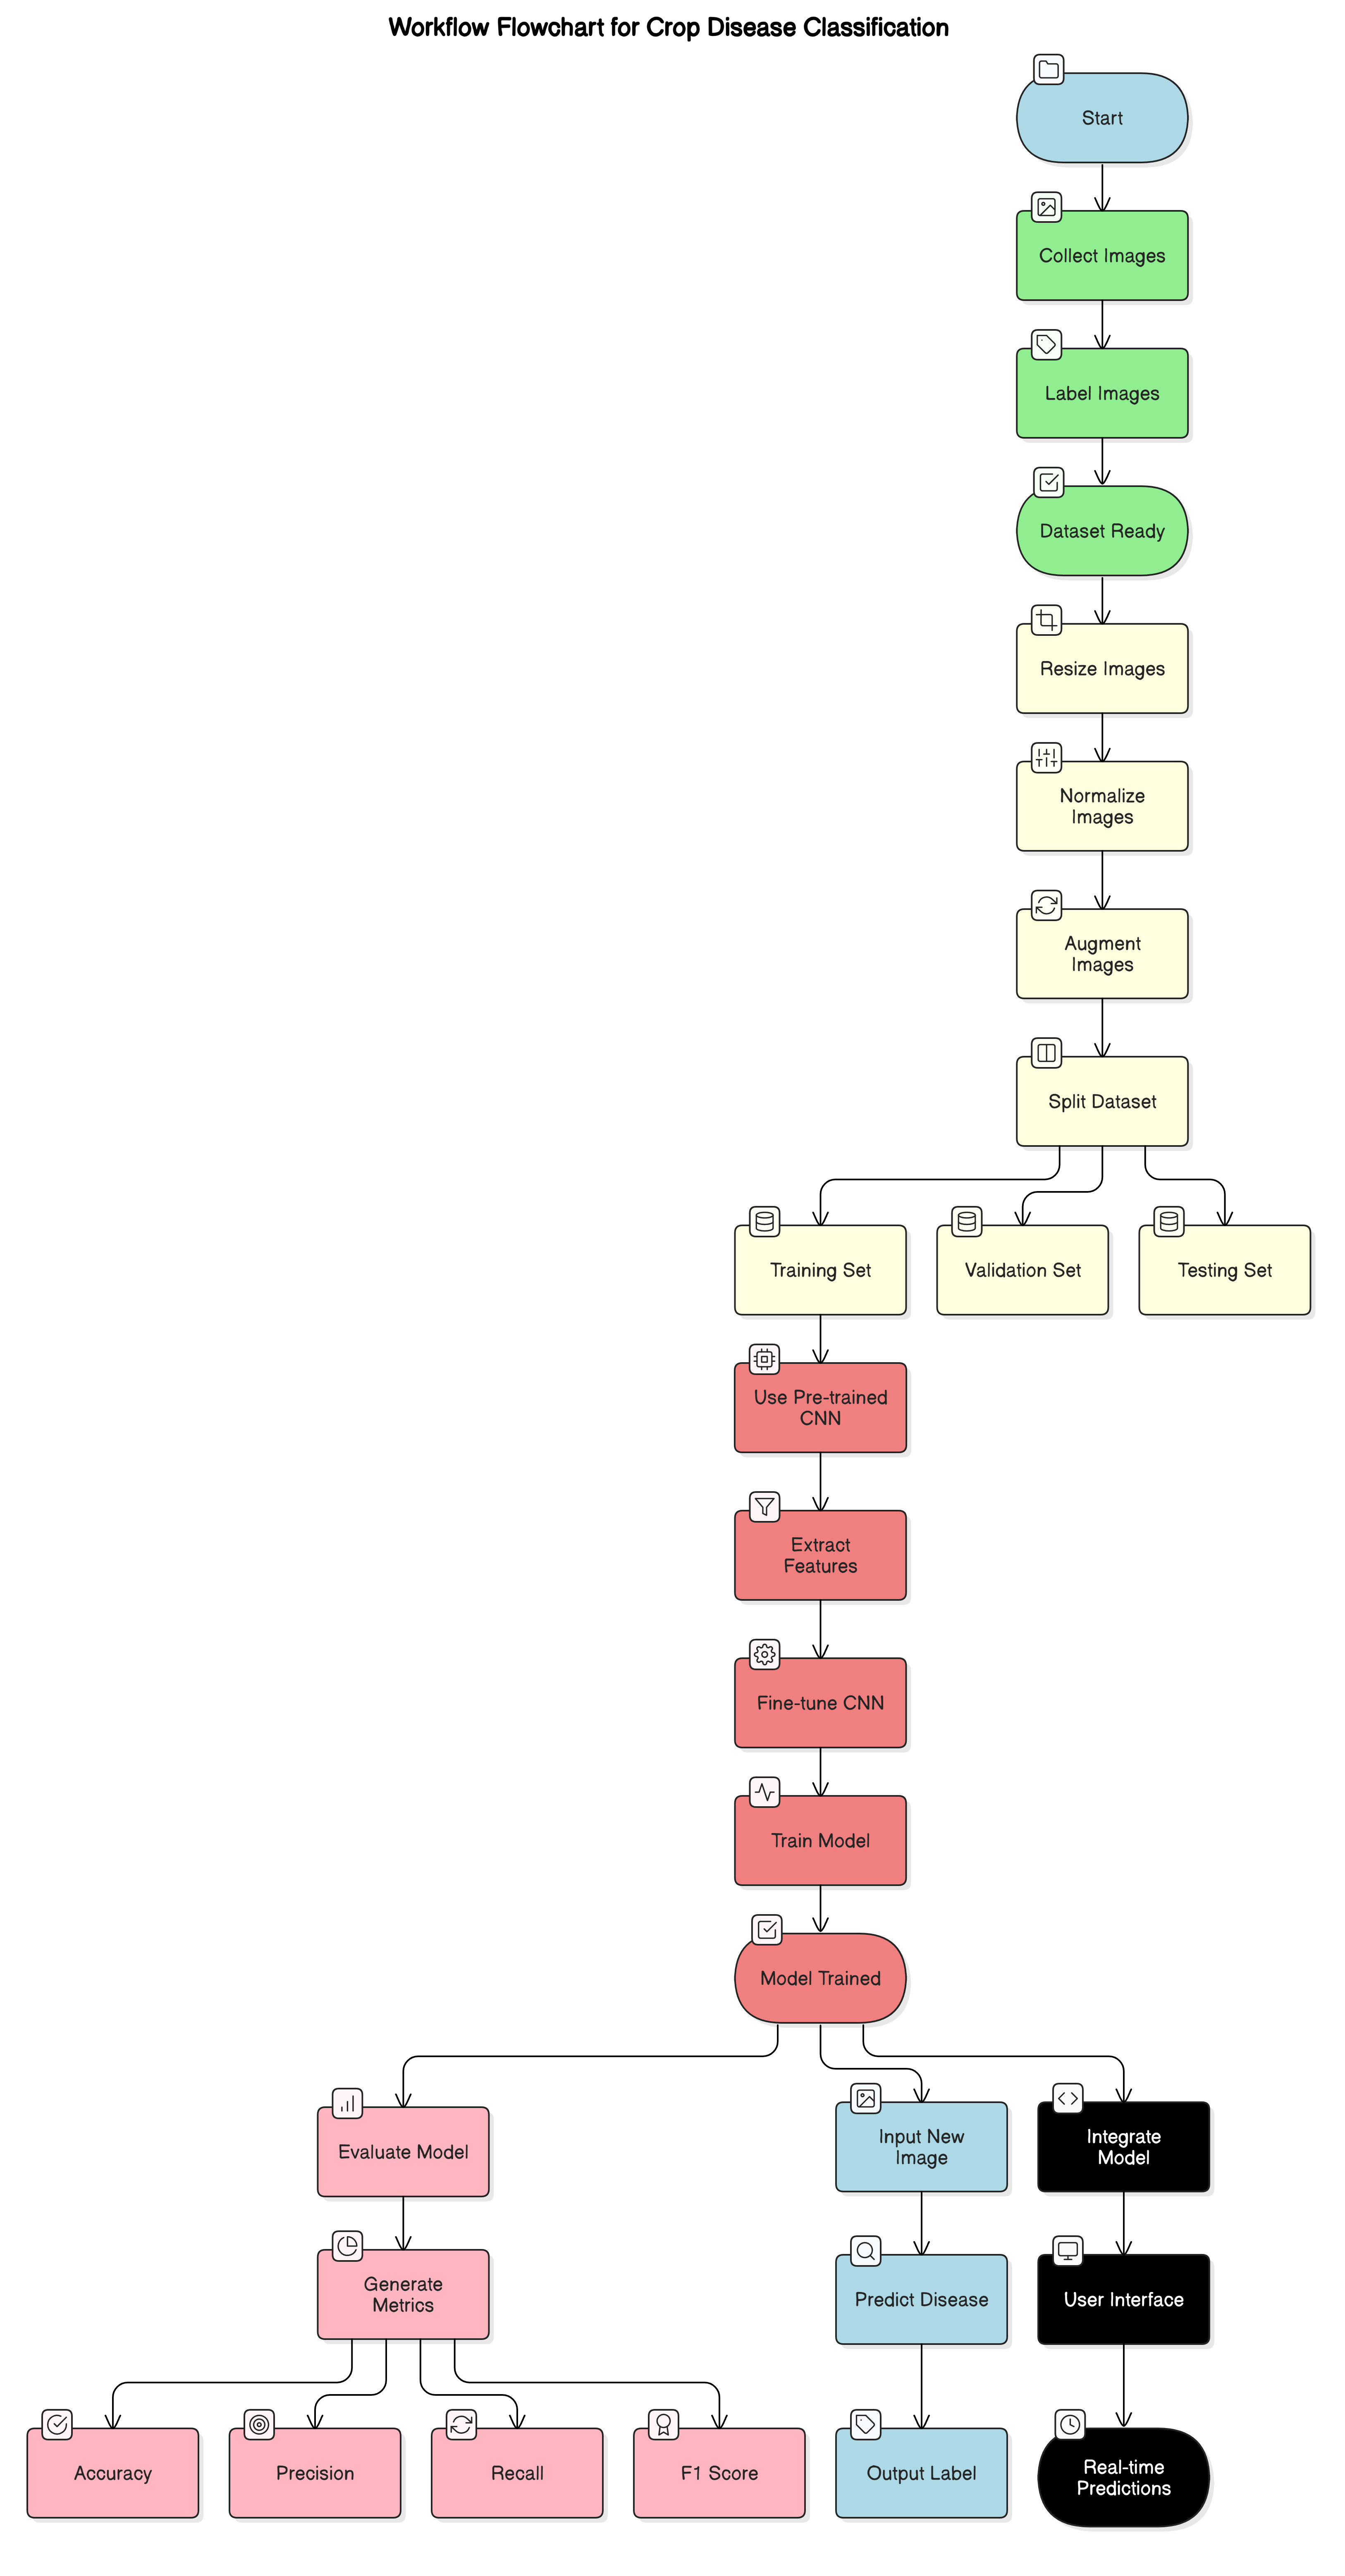
\includegraphics[width=0.5\linewidth]{Images/flow.png}
    \caption{Workflow for Crop Disease Prediction System}
    \label{fig:methodology_workflow}
\end{figure}

\subsection{Cost-Benefit Analysis}
A sample cost-benefit analysis of the project is presented in Table~\ref{tab:cost-benefit}.

\begin{table}[h]
    \centering
    \caption{Sample Cost-Benefit Analysis of the Proposed Project}
    \begin{tabular}{@{}llcc@{}}
        \toprule
        \textbf{Item} & \textbf{Description} & \textbf{Cost (\$)} & \textbf{Benefit (\$)} \\ \midrule
        Development Costs & Software Development & 15,000 & - \\
        Hardware Costs & Servers and Equipment & 5,000 & - \\
        Training Costs & User Training Sessions & 2,000 & - \\
        Maintenance Costs & Annual Maintenance & 1,000 & - \\
        \midrule
        \textbf{Total Costs} &  & \textbf{23,000} & - \\ \midrule
        Increased Efficiency & Time Savings & - & 30,000 \\
        Improved User Satisfaction & User Feedback & - & 10,000 \\
        Revenue Increase & New Customers & - & 20,000 \\
        \midrule
        \textbf{Total Benefits} &  & - & \textbf{60,000} \\ \midrule
        \textbf{Net Benefit} &  & \textbf{23,000} & \textbf{37,000} \\ 
        \bottomrule
    \end{tabular}
    \label{tab:cost-benefit}
\end{table}

\subsection{Gantt Chart}
To plan and track the timeline for the project phases, a Gantt chart will be created using tools like \url{https://www.onlinegantt.com/#/gantt}. The Gantt chart will detail each phase's start and end dates, milestones, and dependencies.
